\documentclass{beamer}
\usetheme{metropolis} % Use metropolis theme

\title{ECON 3818: Introduction to Statistics with Computer Applications}
%\subtitle
\date{\today}
\author{Kyle Butts}

\definecolor{blue}{RGB}{0,114,178}
\definecolor{red}{HTML}{EB0E09}
\definecolor{yellow}{RGB}{240,228,66}
\definecolor{green}{RGB}{0,158,115}
\definecolor{maroon}{HTML}{AF3335}
\definecolor{purple}{HTML}{7E90B8}

\definecolor{mybackground}{HTML}{ECECEC}
\setbeamercolor{background canvas}{bg= mybackground}

\definecolor{buff-gold}{HTML}{CFB87C}
\definecolor{buff-grey}{HTML}{565A5C}
\definecolor{buff-lightgrey}{HTML}{A2A4A3}
\definecolor{buff-black}{HTML}{000000}

\setbeamercolor{alerted text}{fg=buff-gold!80!black}
\setbeamercolor{frametitle}{bg=buff-black}
\setbeamercolor{title}{fg=buff-grey}
\setbeamercolor{button}{bg=buff-gold}

% Allow to remove indent w/ \begin{itemize}[leftmargin= *]
\usepackage{enumitem}
\setlist[itemize]{label= \textbullet}

% \usepackage[libertine]{newtxmath}
\usepackage{longtable}
\usepackage{booktabs}
\usepackage{enumitem}


\begin{document}

% Title Page ---------------------------------------
\maketitle




% Chapter 13 ---------------------------------------
\section{Chapter 13: General Rules of Probability}
\begin{frame}{Basic Rules of Probability}
	
	$A$ is an event/outcome and $P(A)$ is the probability of that outcome, and $S$ is that state space
	\begin{itemize}
		
		\item $0 \leq P(A) \leq 1$ for all $A \in S$
		      
		\item $P(S)=1$
		      
		\item If $A$ and $B$ are disjoint events $\implies$ \[
			P(A \cup B) = P(A) + P(B)
		\]
		      
		\item $P(A^c) = 1 - P(A)$
	\end{itemize}
	
\end{frame}

\begin{frame}{Disjoint versus Not Disjoint}
	
	Using Venn diagrams can help us visualize each of the probability rules
	
	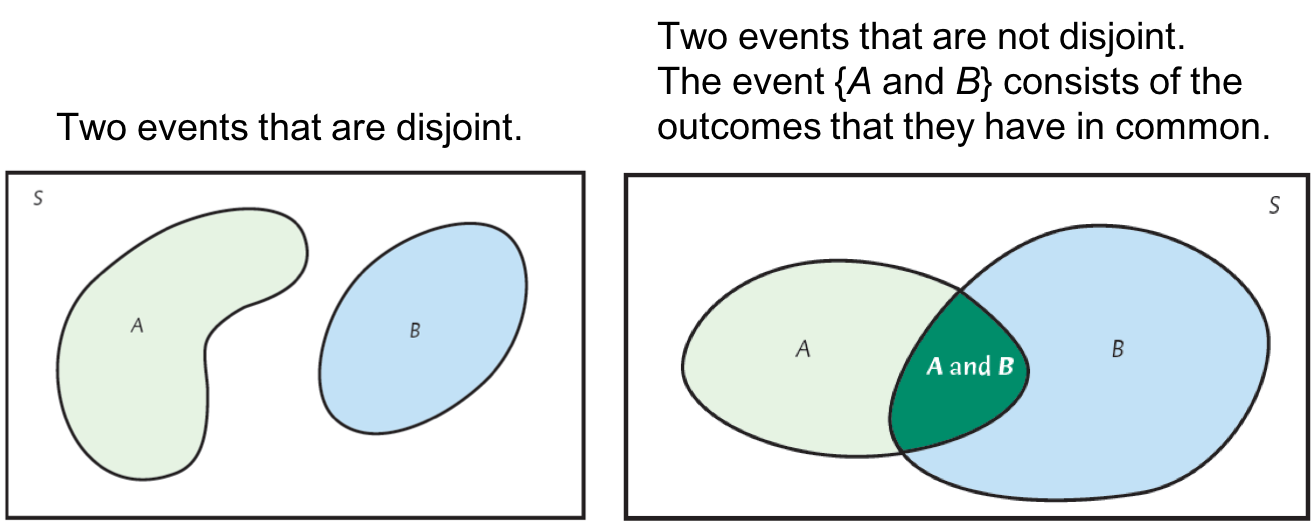
\includegraphics[width=\textwidth]{venndiagram}
\end{frame}

\begin{frame}{General Addition Rule}
	
	\begin{itemize}
		\item If A and B are disjoint events: P(A $\cup$ B)=P(A)+P(B)
		      
		\item For any two events (not necessarily disjoint): \[
			P(A \cup B) = P(A) + P(B)- P(A \cap B)
		\] 

		\item Why does this make sense? What is $A \cap B$ when $A$ and $B$ are disjoint?
	\end{itemize}
	
\end{frame}

\begin{frame}{Venn Diagram Example}
	\begin{centering}
		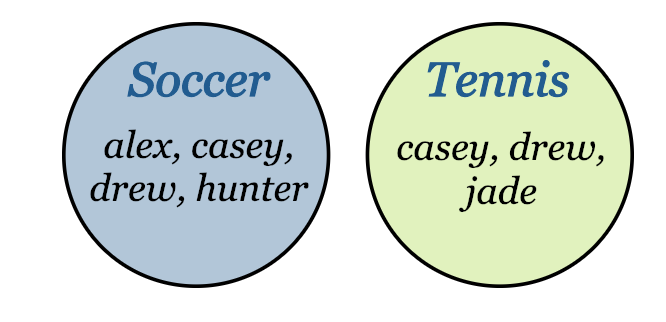
\includegraphics[height=0.25\textwidth]{vd1}
		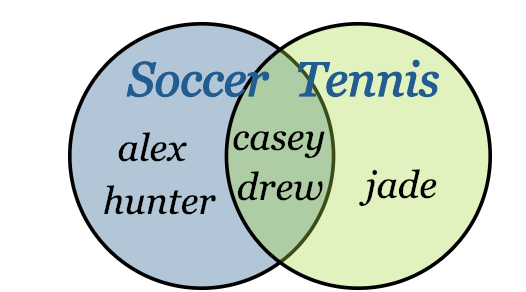
\includegraphics[height=0.25\textwidth]{vd2}
	\end{centering}
	
	\small{
		If we want to find Soccer $\cup$ Tennis ... \\
		Soccer + Tennis = Alex, Casey, Drew, Hunter, Casey, Drew, Jade \\
		
		Soccer $\cap$ Tennis = Casey, Drew\\
		
		Soccer $\cup$ Tennis = Soccer + Tennis - (Soccer $\cap$ Tennis)}\\
	\hspace{30mm}= Alex, Casey, Drew, Hunter, Jade
\end{frame}

\begin{frame}{Clicker Question}
	\begin{centering}
		Let P(A) = 0.4, P(B) = 0.3, and P(A$\cap$B)=0.1
	\end{centering}
	\\
	What is P(A$\cup$B)
	\begin{enumerate}[label=(\alph*)]
		\item 1.1
		\item 0.9
		\item 0.3
		\item 0.6
	\end{enumerate}
\end{frame}



\begin{frame}{Independence}
	
	\begin{itemize}
		\item Two events, A and B, are \alert{independent} if knowing that one occurs does not change the probability that the other occurs
			\begin{itemize}
		      	\item Die lands on a 4 \& Broncos win the Super Bowl
		      	\item Club is drawn from deck of cards \& You get an A on the final exam
			\end{itemize}
		
		\item If A and B are independent: \[
		    P(A \cap B) = P(A)P(B)
		\]	
	\end{itemize}
\end{frame}

\begin{frame}{Clicker Question}
	
	\begin{centering}
		Let P(A) = 0.4, P(B) = 0.3, and P(A$\cap$B)=0.1
	\end{centering}
	\\
	Which of the following statements is true:
	\begin{enumerate}[label=(\alph*)]
		\item A and B are independent because $P(A \cap B) = P(A)P(B)$
		\item A and B are independent because $P(A \cap B) \neq P(A)P(B)$
		\item A and B are not independent because $P(A \cap B) = P(A)P(B)$
		\item A and B are not independent because $P(A \cap B) \neq P(A)P(B)$
	\end{enumerate}
	
\end{frame}

\begin{frame}{Independent vs. Disjoint}
	
	\begin{itemize}
		\item Two events being independent is \alert{NOT} the same as them being disjoint:
		\begin{itemize}
			\item Say event A is being 18 or over, and B is under 18
			
			\item I cannot be both 18 or over, and under 18. This means A and B are \textit{disjoint}
			
			\item If I am not 18 or over, then I am under 18. That means if A isn't true then B must be true. 
				
			\item Since event A tells me about event B, A and B are \textit{not independent}
		\end{itemize}
	\end{itemize}
	
\end{frame}

\begin{frame}{Conditional Probability}
	
	\begin{itemize} 
		\item Sometimes one event occurring tells us something about the probability of a different event
		\item \alert{Conditional probability}: probability of an event, A, given that another event, B, has already occurred
	\end{itemize}
	$$P(A | B)= \frac{P(A \cap B)}{P(B)}$$
	
\end{frame}

\begin{frame}{Visualizing Conditional Probability}
	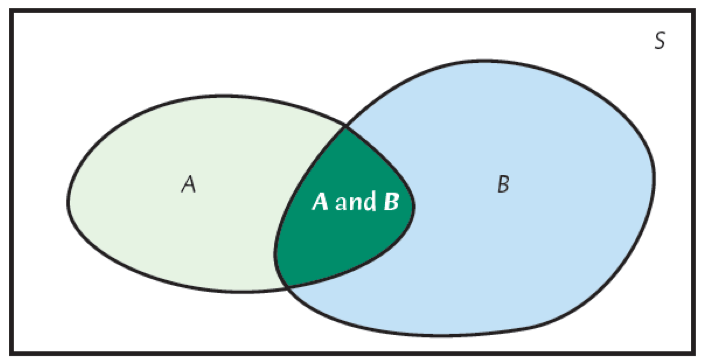
\includegraphics[width=0.85\textwidth]{simplevenndiagram} \\
	You throw a dart and land in $B$. What is the probability that you landed in $A$ as well? $P(A \vert B)$. We can now think of $B$ as the sample space which changes our likelihood of landing in $A$.
\end{frame}

\begin{frame}{Conditional Probability versus Intersection}
	\begin{itemize}
		\item P(work in tech job $\cap$ live in Boulder) vs. \\ P(work in tech job $\vert$ live in Boulder)
		      \begin{itemize}
		      	\item P(work in tech) = work in tech/entire US population = relatively small, let's say 7\%
		      	\item P(live in Boulder) = Boulder population/entire US population = also small, $<$1\%
		      \end{itemize}
		\item This means the probability of BOTH happening is small, because both events are unlikely compared to the \textbf{state space of the entire US population}
		\item But the P(work in tech $|$ live in Boulder) will be higher because now the \textbf{state space is Boulder population}, which has a greater concentration of high-tech employees
	\end{itemize}
\end{frame}




\begin{frame}{Identifying Conditional Probabilities}
	In Colorado, the DMV identifies individuals as having either blonde, brunette or red hair. It also has eyes color. For each of the following statements, check ``True" if it is describing a conditional probability.
	
	\begin{center}
		\begin{tabular}{|c|c|c|}
			\hline
			True & False & Statement                                        \\
			\hline
			     &       & 2.1\% of the drivers are redheads with blue eyes \\
			\hline
			     &       & 45\% of blondes have blue eyes                   \\
			\hline
			     &       & 51\% of people have brown hair or brown eyes     \\
			\hline
			     &       & 77\% of the population is brunette               \\
			\hline 
			     &       & 4.7\% of people with blue eyes are redheads.     \\
			\hline
		\end{tabular}
	\end{center}
\end{frame}

\begin{frame}{Clicker Question}
	Lactose intolerance causes difficulty digesting dairy products that contain lactose. It is particularly common among people of African and Asian ancestry. In the United States, 82\% of the population is white, 14\% is black, and 4\% is Asian. Moreover, 15\% of whites, 70\% of blacks, and 90\% of Asians are lactose intolerance.
	\vskip.2in
	Which of the following statements is true?
	\vskip.2in
	\begin{enumerate}[label=(\alph*)]
		\item P(Asian $\cap$ Lactose Intolerant) = 0.9
		\item P(Asian $|$ Lactose Intolerant) = 0.9
		\item P(Lactose Intolerant $|$ Asian) = 0.9
		\item P(Asian $\cup$ Lactose Intolerant) = 0.9
	\end{enumerate} 
\end{frame}

\begin{frame}{Calculating Conditional Probability: Example}
	
	Consider light truck and car sales in the U.S.:

	\begin{center}
		\begin{tabular}{|l|c|c|c|}
			\hline
			& \textbf{Domestic} & \textbf{Imported} & \textbf{Total} \\ \hline \hline
			Light Truck & 712,700 & 187,000 & 899,700 \\ \hline 
			Car & 472,100 & 155,500 & 627,600 \\ \hline 
			Total & 1,184,800 & 342,500 & 1,527,300 \\ \hline
		\end{tabular}
	\end{center}
		
	If we consider \textit{only cars}, what is the likelihood of a randomly selected sale being a domestic vehicle?

	\small{\[
		P(\text{domestic } \vert \text{ car}) = \frac{P(\text{domestic and car)}}{P(\text{car})} = \frac{\frac{472,100}{1,527,300}}{\frac{627,600}{1,527,300}}=\frac{472,100}{627,600}=0.75
	\]}
	
\end{frame}

\begin{frame}{General Multiplication Rule}
	
	Can use the equation for conditional probability to find the probability of two events happening together:
	$$P(A|B)=\frac{P(A\cap B)}{P(B)}$$
	If we multiply both sides by P(B) we get:
	$$P(A\cap B)=P(B)P(A|B)$$
	
\end{frame}

\begin{frame}{Clicker Question}
	Lactose intolerance causes difficulty digesting dairy products that contain lactose. It is particularly common among people of African and Asian ancestry. In the United States, 82\% of the population is white, 14\% is black, and 4\% is Asian. Moreover, 15\% of whites, 70\% of blacks, and 90\% of Asians are lactose intolerance.
	\vskip.2in
	What is the probability an individual is Asian and lactose intolerant? 
	\vskip.2in
	\begin{enumerate}[label=(\alph*)]
		\item 0.036
		\item 0.044
		\item 0.9
		\item 0.004
	\end{enumerate}
\end{frame}

\begin{frame}{Conditional Probability and Independence}
	
	\begin{itemize}
		\item If P(A) = P(A|B), the probability of A is the same conditional on B or not, then the two events A and B are \alert{independent}
	\end{itemize}
	
\end{frame}

\begin{frame}{Clicker Question}
	Recall we calculated the probability of a car being domestic is 0.75. 
	
	One event is that the vehicle is a car, another event is that the vehicle is domestic. Are these two events independent? 
	
	\begin{center}
		\begin{tabular}{|l|c|c|c|}
			\hline
			& \textbf{Domestic} & \textbf{Imported} & \textbf{Total} \\ \hline \hline
			Light Truck & 712,700 & 187,000 & 899,700 \\ \hline 
			Car & 472,100 & 155,500 & 627,600 \\ \hline 
			Total & 1,184,800 & 342,500 & 1,527,300 \\ \hline
		\end{tabular}
	\end{center}

	\begin{enumerate}[label=(\alph*)]
		\item Yes, they are independent
		\item No, they are not independent
	\end{enumerate}
\end{frame}

\begin{frame}{Law of Total Probability}
	Suppose we partition sample space into n different parts, $B_1, B_2, ..., B_n$\\
	If there is an event A, we can calculate its probability by adding all of its intersections with $B_i$'s
	\begin{center}
		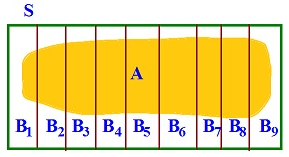
\includegraphics[width=0.6\textwidth]{totalprob}
	\end{center}
	$$P(A)=\sum_{i=1}^nP(A \cap B_i)$$
\end{frame}

\begin{frame}{Law of Total Probability}
	
	$$P(A)=\sum_{i=1}^nP(A \cap B_i)$$
	Use the multiplication rule to show:
	$$P(A)=\sum_{i=1}^n P(A \cap B_i) = \sum_{i=1}^n P(A|B_i)P(B_i)$$
	
\end{frame}

\begin{frame}{Law of Total Probability}
	
	The \alert{Law of Total Probability} says that we can calculate the probability of any event by partitioning the entire sample space into disjoint events and calculating the probabilities of those disjoint events, multiply those by the conditional probabilities, and add them all together.
	\begin{itemize}
		\item Use the law of total probability when you don't know the probability of an event, but you know its occurrence under several disjoint scenarios and the probability of each scenario
	\end{itemize}
	
\end{frame}

\begin{frame}{Midterm Example}
	Let A be the event that a flight from New York to San Francisco arrives on time, and let B be the event that it is a clear day in San Francisco.
	
	Suppose the probability of a clear day is $P(B)=0.6$, We also know that the probability that a plane arrives on a sunny day is 0.9, and on a cloudy day it is 0.5
	
	\begin{enumerate}[label=(\alph*)]
		\item What is the probability that the plan lands on time and it is a sunny day?
		\item What is the probability that the plane lands on time and it is \textit{not} a sunny day?
		\item What is the probability the plan does not land on time?
	\end{enumerate}
\end{frame}

\begin{frame}{Clicker Question}
	Lactose intolerance causes difficulty digesting dairy products that contain lactose. It is particularly common among people of African and Asian ancestry. In the United States, 82\% of the population is white, 14\% is black, and 4\% is Asian. Moreover, 15\% of whites, 70\% of blacks, and 90\% of Asians are lactose intolerance.
	
	What percent of the entire population is lactose intolerant? 
	
	\begin{enumerate}[label=(\alph*)]
		\item 22.5\%
		\item 25.7\%
		\item 0.04\%\
		\item 0.036\%
	\end{enumerate}
\end{frame}
\begin{frame}{Bayes' Law}
	
	\alert{Bayes Law}: gives us a different way to calculate conditional probabilities 
	Let $B_1, B_2, ..., B_n$ be a partition of S. Let A be an event in S. Then:
	$$P(B_i|A)=\frac{P(A|B_i)P(B_i)}{P(A|B_1)P(B_1)+P(A|B_2)P(B_2)+...+P(A|B_n)P(B_n)}$$
	\begin{itemize}
		\item Bayes rule is used to "flip" a conditional probability 
	\end{itemize}
	
\end{frame}

\begin{frame}{Bayes' Law: Example}
	
	Suppose testing for a disease is 99\% accurate, and 0.5\% of people have the diseases. What is the probability that you have the disease, given that the test was positive?
	
	\small{\[ 
		P(Sick \vert Positive) = \frac{P(Positive \vert Sick)P(Sick)}{P(Positive \vert Sick)(Sick) + P(Positive \vert Healthy)P(Healthy)}
	\]}
	
	\small{\[ 
		P(Sick \vert Positive)= \frac{0.99*0.005}{(0.99*0.005)+(0.01*0.995)} = 0.332
	\]}
	
\end{frame}


% \begin{frame}{Bayesian Updating}
%	The power of Bayes' Law is in \alert{Bayesian updating}
%	\begin{itemize}
%		\item Choose \alert{prior} probability, $P(B_i)$
%		\item Calculate the \alert{posterior} probability, $P(B_i|A)$, using Bayes' Law where A is the current state of the world
%		\item Use the posterior probability as the new prior probability and repeat
%	\end{itemize}
%	This iterative process leads to you closer to the true value based on the evidence around you
% \end{frame}
%
% \begin{frame}{Clicker Question}
%	Say we determined that the large number of positive results could be due to the $P(Sick)$ being greater than 0.5\% For example, let's say that we update our prior of $P(Sick)$ to 1\%. What will happen to the probability that a positive results correctly identifies individual with the disease, $P(Sick|Positive)$
%	
%	\begin{enumerate}[label=(\alph*)]
%		\item $P(Sick|Positive)$ stays the same 
%		      \item$P(Sick|Positive)$ decreases
%		      \item$P(Sick|Positive)$ increases
%	\end{enumerate}
% \end{frame} 






\end{document}